% Editable source for the C++ container classification diagram.
% From this directory, regenerate with:
% latex -interaction=nonstopmode -halt-on-error container-1.tex
% dvisvgm --no-fonts --exact --bbox=papersize -o container-1.svg container-1.dvi
\documentclass[tikz,border=4pt]{standalone}
\usepackage{lmodern}
\usetikzlibrary{arrows.meta,backgrounds}

\begin{document}
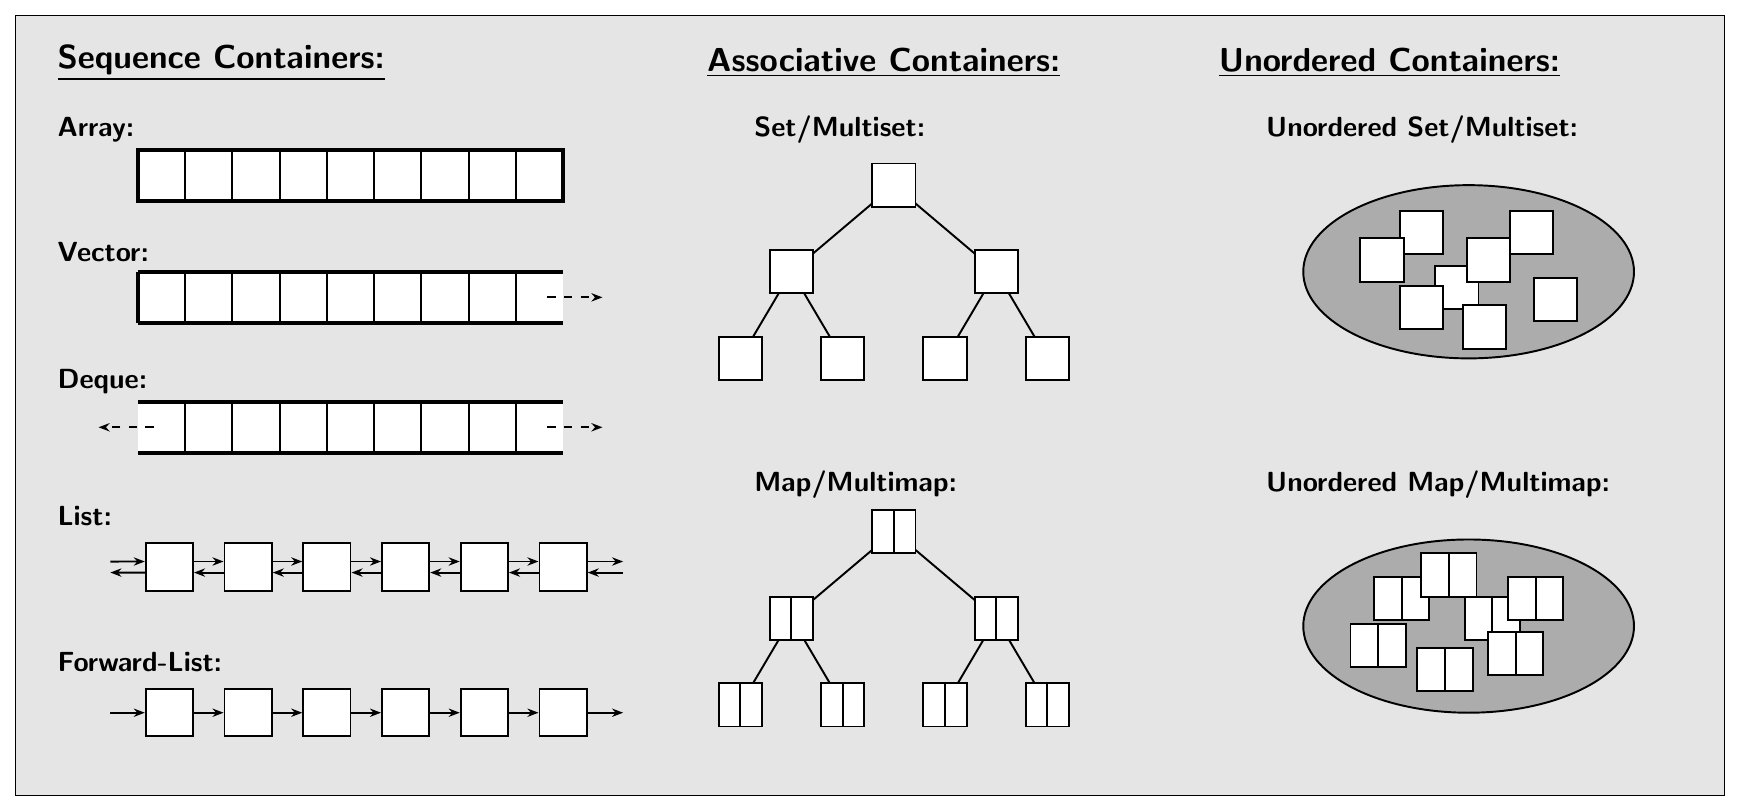
\begin{tikzpicture}[
    x=1cm,y=-1cm,line width=0.7pt,
    font=\sffamily,
    >={Stealth[length=4pt]},
    heading/.style={anchor=west,font=\sffamily\bfseries\large},
    label/.style={anchor=west,font=\sffamily\bfseries},
    element/.style={rectangle,draw,fill=white,minimum size=5.5mm,inner sep=0pt},
    background rectangle/.style={fill=gray!20,draw=black},
    show background rectangle
  ]
  \path[use as bounding box] (0,0) rectangle (21.4,9.6);

  \node[heading] at (0.25,0.45) {\underline{Sequence Containers:}};
  \node[heading] at (8.5,0.45) {\underline{Associative Containers:}};
  \node[heading] at (15,0.45) {\underline{Unordered Containers:}};

  % Fixed-size array: both ends are closed.
  \node[label] at (0.25,1.3) {Array:};
  \foreach \i in {0,...,8} {
    \draw[fill=white] ({1.4+0.6*\i},1.55) rectangle ++(0.6,0.65);
  }
  \draw[line width=1.4pt] (1.4,1.55) rectangle (6.8,2.2);

  % Vector: extension at the back. Deque: extension at both ends.
  \foreach \y/\name in {3.1/Vector,4.75/Deque} {
    \node[label] at (0.25,\y-0.25) {\name:};
    \fill[white] (1.4,\y) rectangle (6.8,\y+0.65);
    \draw[line width=1.4pt] (1.4,\y) -- (6.8,\y)
      (1.4,\y+0.65) -- (6.8,\y+0.65);
    \foreach \i in {1,...,8}
      \draw ({1.4+0.6*\i},\y) -- ++(0,0.65);
    \draw[dashed,->] (6.6,\y+0.325) -- (7.3,\y+0.325);
  }
  \draw[line width=1.4pt] (1.4,3.1) -- (1.4,3.75);
  \draw[dashed,->] (1.6,5.075) -- (0.9,5.075);

  % Lists: paired arrows for list, forward arrows for forward_list.
  \node[label] at (0.25,6.2) {List:};
  \node[label] at (0.25,8.05) {Forward-List:};
  \foreach \y/\prefix in {6.85/list,8.7/forward} {
    \foreach \i in {0,...,5}
      \node[element,minimum size=6mm] (\prefix-\i) at ({1.8+\i},\y) {};
  }
  \foreach \i [evaluate=\i as \j using int(\i+1)] in {0,...,4} {
    \draw[->] ([yshift=2pt]list-\i.east) -- ([yshift=2pt]list-\j.west);
    \draw[<-] ([yshift=-2pt]list-\i.east) -- ([yshift=-2pt]list-\j.west);
    \draw[->] (forward-\i.east) -- (forward-\j.west);
  }
  \draw[->] (1.05,6.78) -- ([yshift=2pt]list-0.west);
  \draw[<-] (1.05,6.92) -- ([yshift=-2pt]list-0.west);
  \draw[->] ([yshift=2pt]list-5.east) -- ++(0.45,0);
  \draw[<-] ([yshift=-2pt]list-5.east) -- ++(0.45,0);
  \draw[->] (1.05,8.7) -- (forward-0.west);
  \draw[->] (forward-5.east) -- ++(0.45,0);

  % Ordered sets store single elements; ordered maps store key/value pairs.
  \node[label] at (9.1,1.3) {Set/Multiset:};
  \node[label] at (9.1,5.8) {Map/Multimap:};
  \foreach \y/\prefix in {2.0/set,6.4/map} {
    \coordinate (\prefix-root) at (11,\y);
    \coordinate (\prefix-left) at (9.7,\y+1.1);
    \coordinate (\prefix-right) at (12.3,\y+1.1);
    \coordinate (\prefix-ll) at (9.05,\y+2.2);
    \coordinate (\prefix-lr) at (10.35,\y+2.2);
    \coordinate (\prefix-rl) at (11.65,\y+2.2);
    \coordinate (\prefix-rr) at (12.95,\y+2.2);
    \draw (\prefix-root) -- (\prefix-left)
      (\prefix-root) -- (\prefix-right)
      (\prefix-left) -- (\prefix-ll)
      (\prefix-left) -- (\prefix-lr)
      (\prefix-right) -- (\prefix-rl)
      (\prefix-right) -- (\prefix-rr);
    \foreach \name in {root,left,right,ll,lr,rl,rr}
      \node[element] at (\prefix-\name) {};
  }
  \foreach \name in {root,left,right,ll,lr,rl,rr}
    \draw ([yshift=2.75mm]map-\name) -- ([yshift=-2.75mm]map-\name);

  % Unordered collections: no ordering links; maps still contain pairs.
  \node[label] at (15.6,1.3) {Unordered Set/Multiset:};
  \draw[fill=gray!65] (18.3,3.1) ellipse (2.1 and 1.1);
  \foreach \x/\y in {17.7/2.6,17.2/2.95,18.15/3.3,18.55/2.95,19.1/2.6,19.4/3.45,18.5/3.8,17.7/3.55}
    \node[element] at (\x,\y) {};

  \node[label] at (15.6,5.8) {Unordered Map/Multimap:};
  \draw[fill=gray!65] (18.3,7.6) ellipse (2.1 and 1.1);
  \foreach \x/\y in {17.45/7.25,18.05/6.95,18.6/7.5,19.15/7.25,18.9/7.95,18.0/8.15,17.15/7.85} {
    \node[element,minimum width=7mm] at (\x,\y) {};
    \draw (\x,\y-0.275) -- (\x,\y+0.275);
  }
\end{tikzpicture}
\end{document}
